\documentclass[]{article}

\usepackage{cite} % Add this line to include the cite package
% \usepackage[backref]{hyperref} % Add this line to include the hyperref package

\usepackage{amsmath} % Add this line to include the amsmath package
\usepackage{graphicx} % Add this line to include the graphicx package
\usepackage{fancyhdr}

\title{Computer Vision homework 2}
\author{Pan Changxun}
\date{March 2025}

\topmargin=-0.45in      %
\evensidemargin=0in     %
\oddsidemargin=0in      %
\textwidth=6.5in   
\textheight=9.0in       %
\headsep=0.25in 

\pagestyle{fancy}
\fancyhf{} % Clear all header and footer fields
\fancyhead[L]{Pan Changxun} % Left header
\fancyhead[C]{Computer Vision homework 2} % Center header
\fancyhead[R]{March 2025} % Right header
%\fancyfoot[L]{\leftmark} % Left footer
\fancyfoot[C]{\thepage} % Center footer
%\fancyfoot[R]{} % Right footer

\begin{document}
\maketitle

\section{Implement SIFT}
In \verb|sift_demo.ipynb|, I show the implementation of SIFT and put it into \verb|sift_useful.py|, showing a demo in \verb|main.py|
Here is the result of SIFT on the image "building2".
\begin{figure}[h]
	\centering
	\begin{minipage}{0.48\textwidth}
		\centering
		\includegraphics[width=\textwidth]{detect_building.png}
		\caption{SIFT result on building2 (original)}
		\label{fig:sift_result}
	\end{minipage}
	\hfill
	\begin{minipage}{0.48\textwidth}
		\centering
		\includegraphics[width=\textwidth]{detect_rotate_building.png}
		\caption{SIFT result on building2 (rotated)}
		\label{fig:sift_result1}
	\end{minipage}
\end{figure}

\begin{figure}[h]
	\centering
	\includegraphics[width=0.90\textwidth]{match_rotate.png}
	\caption{SIFT result on building2}
	\label{fig:sift_result2}
\end{figure}


\newpage
\section{Match With RANSAC}
The effect of RANSAC is shown in the figure below. The left image is the original image, and the right image is the result after RANSAC.
\begin{figure}[h]
	\centering
	\begin{minipage}{0.48\textwidth}
		\centering
		\includegraphics[width=\textwidth]{before_ransac.png}
		\caption{RANSAC before}
		\label{fig:ransac_result}
	\end{minipage}
	\hfill
	\begin{minipage}{0.48\textwidth}
		\centering
		\includegraphics[width=\textwidth]{after_ransac.png}
		\caption{RANSAC result }
		\label{fig:ransac_result1}
	\end{minipage}
\end{figure}


\newpage
\section{Homography}
I use the Homography matrix to transform the image and get the result.
And I obtain 3 distance: 
Using the homography transformation, I calculated the following real-world distances:
\begin{itemize}
	\item Ball to gate: $23.84$ m
	\item Left foot to gatepost: $4.74$ m
	\item Referee to ball: $7.49$ m
\end{itemize}
\begin{figure}[h]
	\centering
	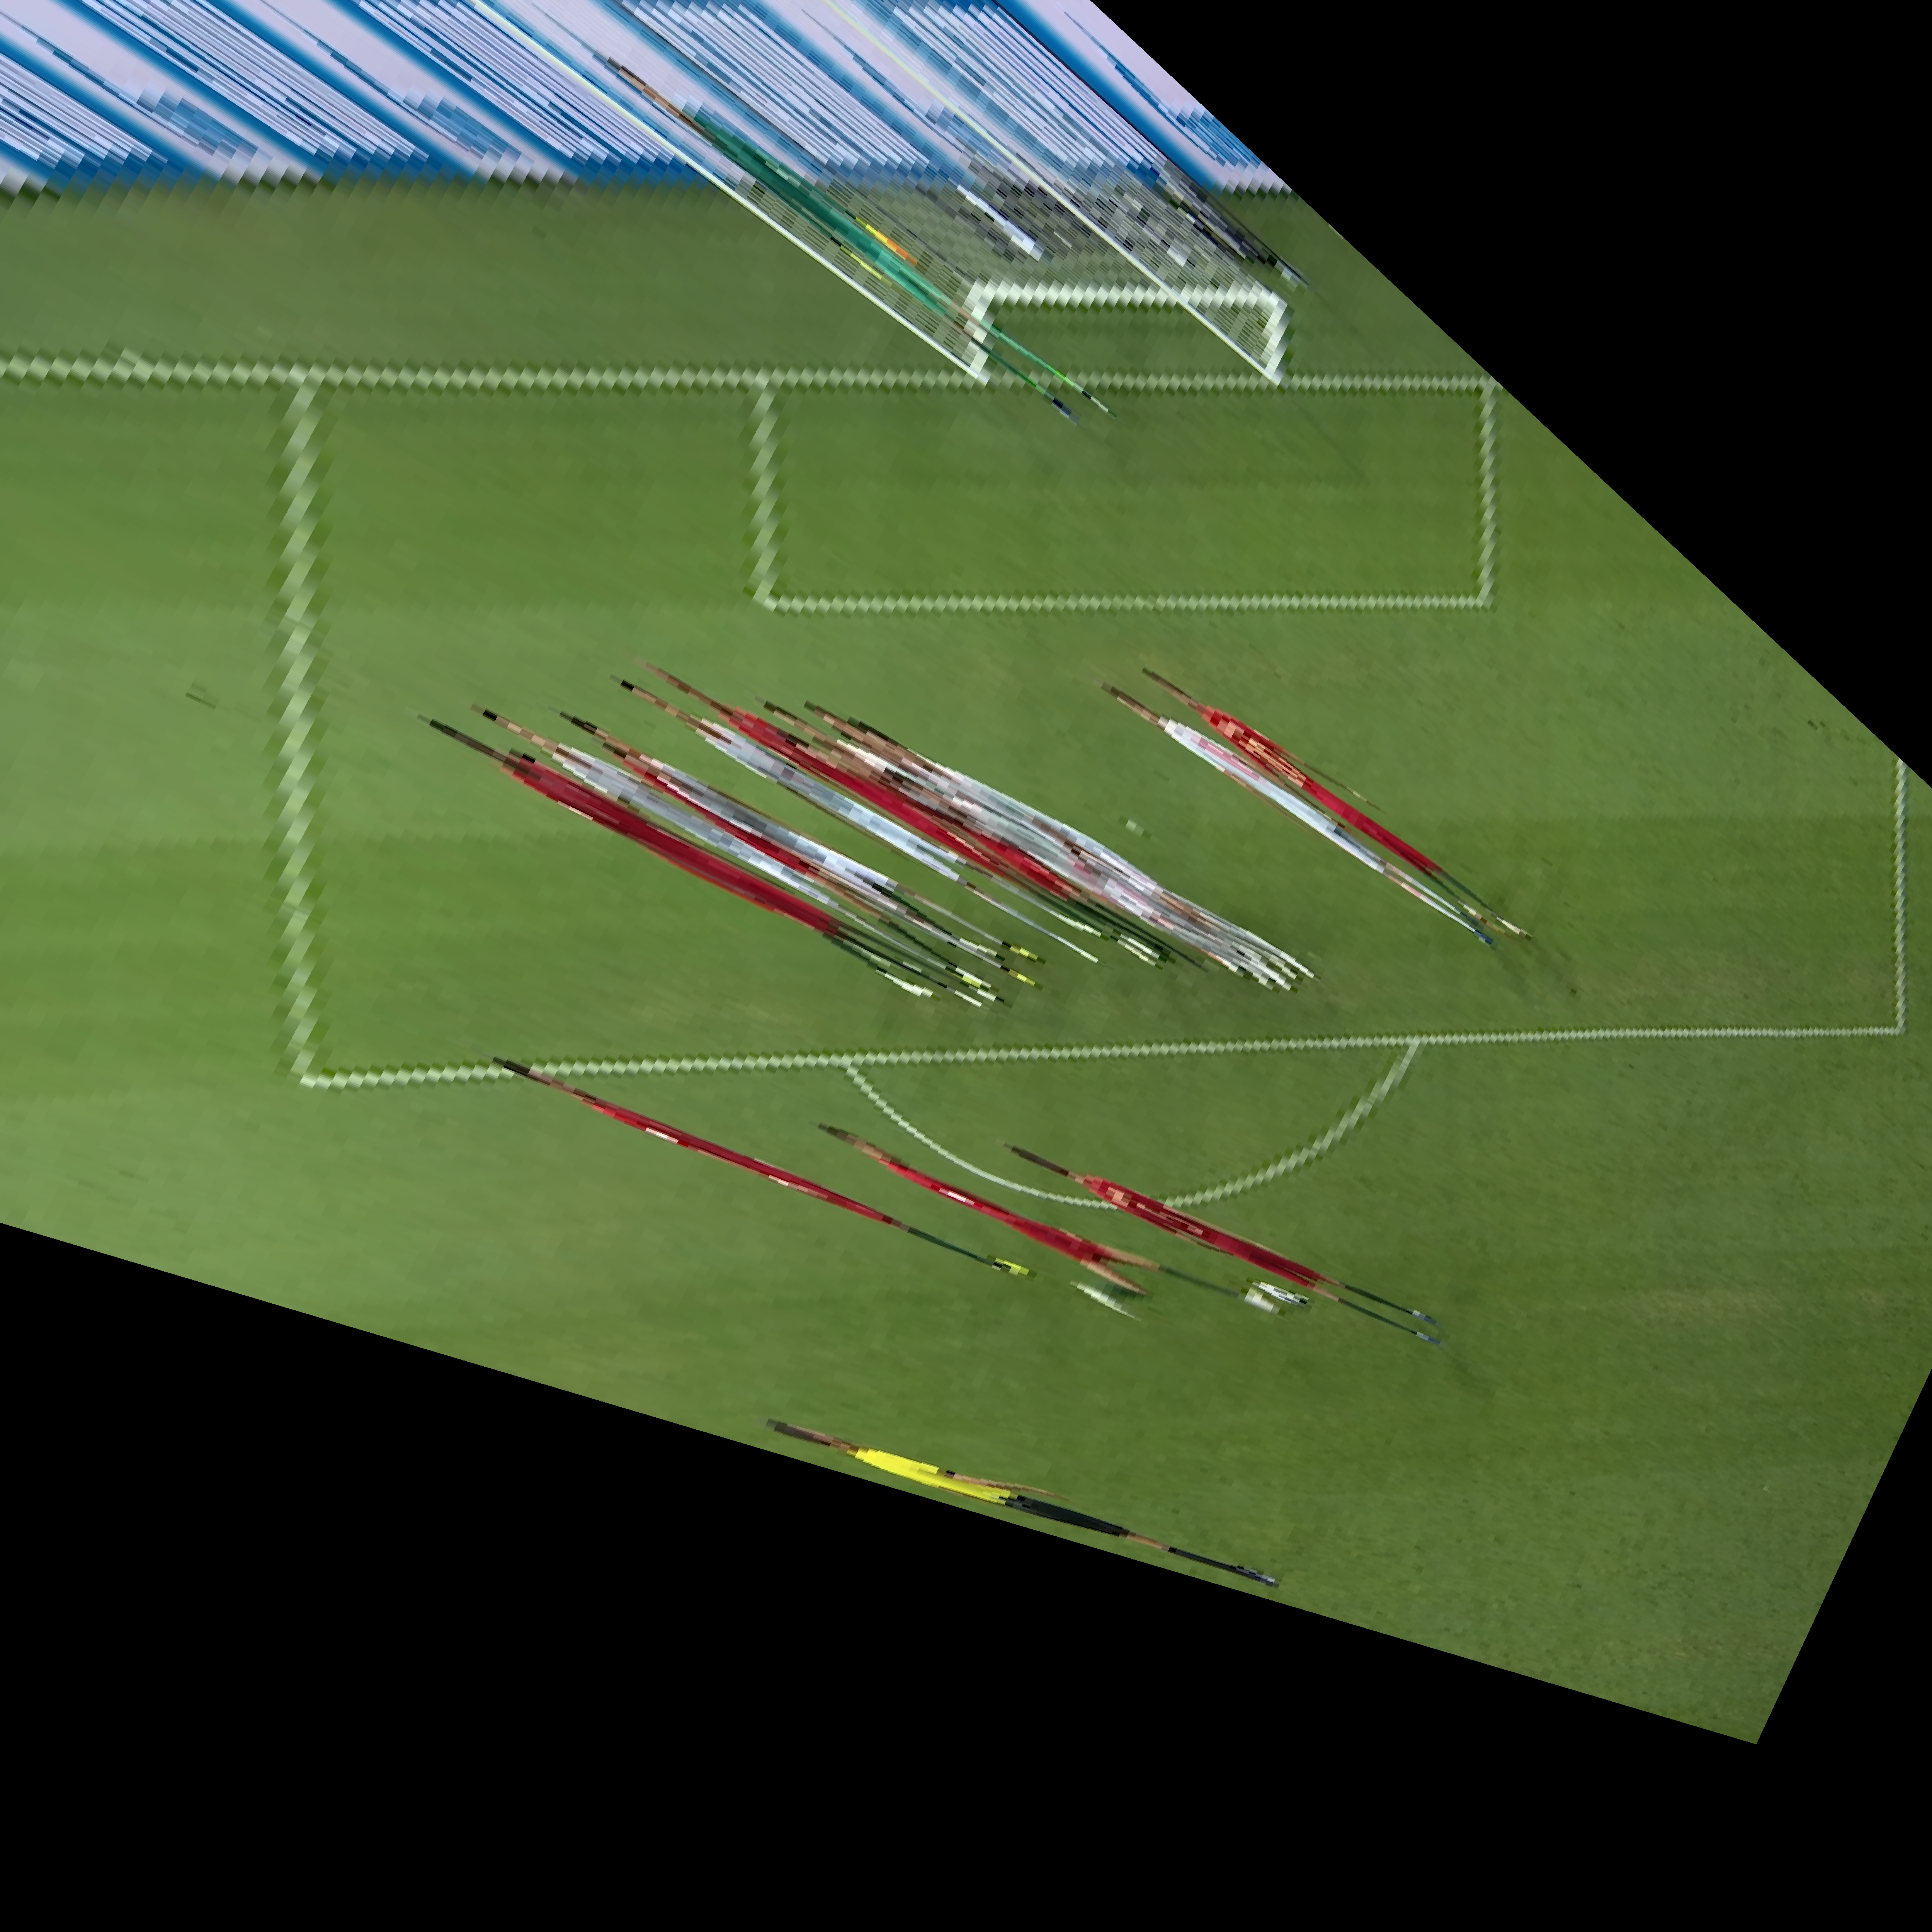
\includegraphics[width=0.90\textwidth]{transformed_result.png}
	\caption{Homography result on football}
	\label{1}
\end{figure}

\newpage
\section{stitch}
I use the SIFT to match the image and do the RANSAC to get the homography matrix.
Then I use the homography matrix to transform the image and get the result. putting building1 and building2 together into blend1., building3 and building4 together into blend2. Then put blend1 and blend2 together into final.
\begin{figure}[h]
	\centering
	\begin{minipage}{0.48\textwidth}
		\centering
		\includegraphics[width=\textwidth]{blend1.png}
		\caption{Stitching result on building1 and building2}
		\label{fig:stitch1}
	\end{minipage}
	\hfill
	\begin{minipage}{0.48\textwidth}
		\centering
		\includegraphics[width=\textwidth]{blend2.png}
		\caption{Stitching result on building3 and building4}
		\label{fig:stitch2}
	\end{minipage}
\end{figure}
\begin{figure}[h]
	\centering
	\includegraphics[width=0.6\textwidth]{panorama.png}
	\caption{Stitching result on building1, building2, building3 and building4}
	\label{fig:stitch3}
\end{figure}

\end{document}